\chapter{Blind reverberation time estimation}
\label{chap:rt60}


% This is the modified v2 as after Emilia's comments

%%%%%%%%%%%%%%%%%%%%%%%%%%%%%%%%%%%%%%%%%%%%%%%%%%%%%%%%%%%%
%%%%%%%%%%%%%%%%%%%%%%%%%%%%%%%%%%%%%%%%%%%%%%%%%%%%%%%%%%%%
\section{Introduction}

%The knowledge about the acoustic properties of an enclosure results of the greatest interest for many situations within the microphone array and acoustic signal processing fields. 
Knowledge about the acoustic properties of an enclosure is a fundamental topic with many applications in the microphone array and acoustic signal processing field.
Problems such as dereverberation \cite{braun2018evaluation} or source separation \cite{gannot2017consolidated} may benefit from this information, 
%or might even require \textit{a priori} acoustic parameter estimations. 
and may require prior estimation of the related parameters.
%Reverberation time $T_{60}$ \cite{kuttruff2016room} might be one of the most widespread acoustic parameters; it represents the time required 
%%for a sound in the diffuse field to decrease its energy envelope by 60 dB. 
%for the reverberant sound field power to decay by 60 dB.
%Reverberation time can be accurately computed from the room geometry \cite{sabine1927collected} or from the Impulse Response (IR) \cite{schroeder1965new}; the problem of $T_{60}$ estimation just from observations of the reverberant signal itself is referred to as the blind reverberation time estimation, and it still remains an open research question.

The 2016 Acoustic Characterisation of Environments (ACE) Challenge \cite{eaton2016estimation} gathered dozens of methods designed for blind $T_{60}$ and Direct-to-Reverberation Ratio (DRR) estimation; nowadays, it is still considered as a state-of-the-art source for 
%method comparison, and the evaluation metrics used have become standard. 
%evaluating performance of BRTE and comparing different methods
performance evaluation and comparison among methods.

Most of the model-based $T_{60}$ estimation algorithms consider the reverberant signal envelope as an exponential decay, so that the problem is reduced to finding a signal offset and estimate the decay rate. 
%For instance, the best scoring $T_{60}$ estimation algorithm, in terms of the Pearson correlation, implements a variant of this idea on the narrowband STFT spectrum \cite{prego2012blind}; this method will be used in next sections as the baseline method. 
Moreover, in last years, data-driven models have outperformed the previous state-of-the-art results \cite{gamper2018blind, looney2020joint, bryan2020impulse}.
%Some representative examples of such approaches are based on multi-layer perceptrons \cite{xiong2018joint} or convolutional neural networks (CNN) \cite{gamper2018blind, looney2020joint, bryan2020impulse}.
A comparative review on single-channel blind $T_{60}$ estimation algorithms was recently published \cite{lollmann2019comparative}. 
%Apart from providing a complete state-of-the-art overview, this work extends the ACE Challenge evaluation to more recent methods.  

However, most of the existing reverberation time estimation methods focus on the single-channel case. A representative example can be drawn from the ACE Challenge, where, despite the fact that one of the reverberant datasets was recorded with an \textit{em32 Eigenmike} spherical microphone array, none of the methods use of it for the $T_{60}$ estimation task. 

%one of the data subsets was recorded with an \textit{em32 Eigenmike} spherical microphone array, featuring 32 capsules. However, only one of the participants \cite{chen2015estimation} made use of those multichannel recordings, but just for the DRR estimation problem. 
%In a slightly different context, the method proposed in \cite{falcon2019machine} estimates reverberation time from room geometry; while the groundtruth values are computed through spatial filtering of Eigenmike recordings, those are just employed for algorithm training. 

On the other hand, recent years have witnessed a growing interest in immersive audio for virtual and augmented reality.
This situation has consolidated Ambisonics as the \textit{de facto} standard for spatial audio. Dedicated spherical microphone arrays have reached the market in last years; their multichannel nature makes possible spatial manipulations that 
%improve traditional signal processing methods.
complement traditional signal enhancement methods.

In this chapter, we present a novel approach to the problem of multichannel blind reverberation time estimation, specifically focusing on first order ambisonic (FOA) recordings. 
%The method is based on dereverberation plus IR estimation by system identification. 
The method is based on a dereverberation stage followed by system identification.
To the best of our knowledge, the proposed algorithm is the first reverberation time estimation method specifically designed for first order ambisonic audio.

The rest of the Chapter is organized as follows. Section~\ref{sec:signalmodel} introduces the nomenclature and the signal model. Sections~\ref{sec:baseline} and \ref{sec:proposed} describe the baseline and the proposed methods, respectively. The experimental setup is described in Section~\ref{sec:experimental}, and the results are discussed in Section~\ref{sec:results}. Finally, a conclusion is presented in Section~\ref{sec:conclusion}.

The research presented in this Chapter has been submitted for publication at the IEEE 22nd International Workshop on Multimedia Signal Processing \cite{rt}.

%%%%%%%%%%%%%%%%%%%%%%%%%%%%%%%%%%%%%%%%%%%%%%%%%%%%%%%%%%%%
%%%%%%%%%%%%%%%%%%%%%%%%%%%%%%%%%%%%%%%%%%%%%%%%%%%%%%%%%%%%
\section{Signal Model}
\label{sec:signalmodel}

Let us consider a FOA signal $x_n^m(t)$, with $M=4$ as the number of channels.
Let us further assume the convolutive mixture signal model described in Eq.~\ref{eq:convolutivemixturemultichannel}, where the reverberant signal $x_n^m(t)$ represents the signal captured by an ideal spherical microphone array located in a reverberant enclosure. 
Let $s(t)$ denote the signal of the only sound source present in the scene, and $h_n^m(t)$ denote the ambisonic RIR modelling the acoustic enclosure:
\begin{equation}
	x_n^m(t) = s(t) \ast h_n^m(t)
\end{equation}

It is important to remark that $T_{60}$ estimation here assumes no receiver directionality. In an ambisonic context, this corresponds to the zeroth order component. Therefore, in what follows, all methods estimating IR parameters will be applied to the zeroth order channel, $x_0(t)$.

%%%%%%%%%%%%%%%%%%%%%%%%%%%%%%%%%%%%%%%%%%%%%%%%%%%%%%%%%%%%
%%%%%%%%%%%%%%%%%%%%%%%%%%%%%%%%%%%%%%%%%%%%%%%%%%%%%%%%%%%%
\section{Baseline method}
\label{sec:baseline}


The baseline algorithm, taken from \cite{prego2012blind}, is based on the detection of abrupt event offsets in the time-frequency domain. The subband energy decay on the transitions can be then used to compute an estimate of the full-band decay. This method performed best in the ACE Challenge regarding the Pearson correlation coefficient between estimated and true $T_{60}$\cite{eaton2016estimation}.

Let us consider the zeroth order channel of the recorded signal, $x_0(t)$, and its Short-Time Frequency Transform (STFT) counterpart $X_0(k,n)$.
%Although the method could be potentially applied to any of the channels, in physical terms it makes more sense to work with an omnidirectional sound field representation; hence the usage of the zeroth order channel.
The \textit{subband energy} $\bar{E}(k,n)$ of the recorded signal can be expressed as:\begin{equation}
	\bar{E}(k,n) = |X_0(k,n)|^2.
\end{equation}

A \textit{Free Decay Region} (FDR) is defined as a group of consecutive bins within the same subband which exhibit a monotonically decreasing energy. 
A FDR search is performed on the subband energy spectrogram $\bar{E}(k,n)$: for each band, the algorithm tries to find at least one FDR, iterartively reducing the FDR length if no candidates are found. 

The next step is the estimation of the reverberation time, which is performed using a subband equivalent of Schroeder's method \cite{schroeder1965new}.
The \textit{Subband Energy Decay Function} (SEDF) associated with a given FDR is computed as:

\begin{equation}
	\bar{c}(k,n) = 10 \log_{10} \frac{\sum_{\nu=n}^{L_c-1} \bar{E}(k,\nu)} {\sum_{\nu=0}^{L_c-1} \bar{E}(k,\nu)} \text{dB},
\end{equation}
where $n = 0 \ldots, L_c-1$ spans the length of the FDR. A linear regression is then performed on each SEDF curve: $T_{60}$ is computed as the time required by the resulting line to reach the $-60 \text{ dB}$ reference.

This procedure yields a $T_{60}$ estimate per FDR. In order to obtain a global estimate, the algorithm proposes a two-step statistical filtering. First, it obtains a narrowband estimate as the median of all estimates within each subband. Then, the resulting broadband value $\bar{T}_{60}$ is computed as the median of all subband estimates.
The last step of the method is the expansion of the resulting dynamic range by a linear mapping. This procedure is required because of the compression introduced by the median operator. The final value $T_{60}$ is thus a linear mapping of $\bar{T}_{60}$, where the parameters $\alpha$ and $\beta$ might be obtained by linear regression on a training stage:
\begin{equation}
	T_{60} = \alpha \bar{T}_{60} + \beta
\label{eq:expansion}
	\end{equation}



%%%%%%%%%%%%%%%%%%%%%%%%%%%%%%%%%%%%%%%%%%%%%%%%%%%%%%%%%%%%
%%%%%%%%%%%%%%%%%%%%%%%%%%%%%%%%%%%%%%%%%%%%%%%%%%%%%%%%%%%%
\section{Proposed method}
\label{sec:proposed}

We propose a novel method for reverberation time estimation, based on two steps: signal dereverberation, and system identification. The main idea consist in obtaining an estimate of the dereverberated signal, which is later used for estimating the multichannel IR given the recorded reverberant signal. The reverberation time can be thus computed by the decay slope of the estimated IR. 

\subsection{Dereverberation}

Let us consider now the \textit{CTF} model (Eq.~\ref{eq:convolutivetransferfunction}) version of the proposed signal model:
\begin{equation}
\label{eq:ctf}
	X_m(k, n) = \sum_{l=0}^{L_h-1} H_m(k, l) S(k, n-l), 
\end{equation} 
where the multichannel filter $H_m(k, l)$ of length $L_h$ contains the \textit{CTF coefficients} between the source and the microphones.

Considering the room impulse response model of Eq.~\ref{eq:directreverberant}, 
it is possible to sequentially split the former expression in the following way:
\begin{equation}
\label{eq:model}
\begin{aligned}
	&X_m(k, n) = D_m(k, n) + R_m(k,n) = \\
	=\sum_{l=0}^{\tau-1} H_m(&k, l) S(k, n-l) + \sum_{l=\tau}^{L_h-1} H_m(k, l) S(k, n-l),
\end{aligned}
\end{equation} 
%\begin{subequations}
%\begin{equation}
%\label{eq:model}
%	X_m(k, n) = D_m(k, n) + R_m(k, n),
%\end{equation} 
%\begin{equation}
%	D_m(k, n) = \sum_{l=0}^{\tau-1} H_m(k, l) S(k, n-l),
%\end{equation} 
%\begin{equation}
%\begin{aligned}
%	R_m(k_n) = \sum_{l=\tau}^{L_h-1} H_m(k, l) S(k, n-l),
%\end{aligned}
%\end{equation} 
%\end{subequations}
where the parameter $\tau$ represents the \textit{mixing time}, which states the transition time between early reflections and late reverberation. 
In other words, the captured signal is divided between a \textit{direct} part $D_m(k, n)$, containing the direct path and the early reflections, and a \textit{reverberant} part $R_m(k, n)$, which mainly contains the diffuse part of the reverberation.

Assuming a Multichannel Auto-Regressive (MAR) model, $R_m(k, n)$ can be expressed as a multichannel Infinite Impulse Response (IIR) filter applied to the recorded signal:
\begin{equation} 
\label{eq:mar}
	R_m(k, n) = \sum_{i=1}^{M} \sum_{l=0}^{L_g-1} X_i(k,n-\tau-l) G_{mi}(k, l),
\end{equation}
where the coefficients $G_{mi}(k,l) \in \mathbb{C}$  model the relation between channels $m$ and $i$, and have a length of $L_g$ frames. 

By grouping all time frames $n = 1 \ldots, N-1$, it is possible to express Eq.~\ref{eq:mar} in vector notation:
\begin{subequations} 
\begin{equation} 
	\bm{R}_m(k) =  \tilde{\bm{X}}_{\tau}(k) \bm{G}_{m}(k),
\end{equation}
\begin{equation} 
	\tilde{\bm{X}}_{\tau}(k) = [ \tilde{\bm{X}}_{\tau,1}(k), \ldots, \tilde{\bm{X}}_{\tau,M}(k)],
\end{equation}
\end{subequations}
where $\tilde{\bm{X}}_{\tau,m}(k)$ is a $N \times L_g$ matrix, and $\bm{R}_m(k)$ and $\bm{G}_{m}(k)$ are column vectors with lengths $N$ and $L_gM$, respectively.

Finally, the expression can be further simplified by omitting the frequency dependence, and by expressing the channels as columns in the vector notation. Substituting this expression in Eq.~\ref{eq:model} leads to the MAR equation:
\begin{equation} 
\label{eq:D}
	\bm{D} = \bm{X} - \tilde{\bm{X}}_{\tau} \bm{G}.
\end{equation}

Here, the dereverberation problem consists in the estimation of the MIMO filter $\bm{G}$, so that the \textit{clean} signal $\bm{D}$ (containing both direct path and early reflections) can be computed.

The algorithm proposed here is based on the method described in \cite{jukic2015group}. In this case, the dereverberation problem is tackled as an optimization problem, considering that the spectrograms of the reverberant signal are less sparse than those of the corresponding \textit{clean}, and ensuring that the inter-channel signal properties are mantained.
%(hence the reference to the \textit{group} sparsity). 
Although the presented method is applied on the whole signal in \textit{batch} mode, alternative \textit{online} methods could be also used, e.g. \cite{braun2016online}.
%Given that this is a \textit{batch} processing algorithm, the whole audio clip is processed at once. Alternative solutions using online MAR models could be also used if required \cite{braun2016online}.

By using \textit{iteratively reweighted least squares} (IRSL) \cite{chartrand2008iteratively}, it can be shown that an iterative solution for the estimation of $\bm{G}$ at the iteration $(i)$ is given by the following expression:

\begin{equation}
\begin{aligned}
	\label{eq:G}
	\bm{G}^{(i)} = ( \tilde{\bm{X}}_{\tau}^H \bm{W}^{(i)} \tilde{\bm{X}}_{\tau} )^{-1} \tilde{\bm{X}}_{\tau}^H \bm{W}^{(i)} \bm{X}, 
\end{aligned}
\end{equation}
 where $\bm{W}^{(i)}$ is a $N \times N$ diagonal matrix whose diagonal values, $w_n^{(i)}$, can be updated as:
\begin{equation}
\begin{aligned}
\label{eq:w}
	w_n^{(i)} = ( \bm{d}_n^{H (i-1)} \bm{\Phi}^{-1 (i-1)} \bm{d}_n^{(i-1)}  )^{ \frac{p-2}{2} } + \epsilon.
\end{aligned}
\end{equation}

In turn, $\bm{d}_n$ represents the rows of $\bm{D}$ arranged as column vectors of length $M$, $\bm{\Phi}$ is the $M \times M$ Spatial Covariance Matrix (SCM) of $\bm{D}$, $\epsilon$ is an arbitrary small positive value, and $p \leq 1$. The computation and update of the SCM matrix is given by:
\begin{equation}
\begin{aligned}
\label{eq:phi}
	\bm{\Phi}^{(i)} = \frac{1}{N} \bm{D}^{T(i)} \bm{W}^{(i)} \bm{D}^{*(i)}.
\end{aligned}
\end{equation}


%It is interesting to notice that, in the original proposal, the SCM matrix is assigned by default to the identity matrix, and its actual estimation is regarded as optional. However, it is known that the SCM matrix is only equal to the identity matrix in the spherical harmonic domain under isotropic noise \cite{epain2016spherical}. Furthermore, the method has also reported a slightly better performance with the SCM estimation.

To conclude the dereverberation method, Eqs.~\ref{eq:D}, \ref{eq:G}, \ref{eq:w} and \ref{eq:phi} can be applied iteratively, starting by updating Eq.~\ref{eq:w}, until convergence is reached: 
\begin{equation}
 \| \bm{D}^{(i)} - \bm{D}^{(i-1)} \|_F / \| \bm{D}^{(i)} \|_F < \eta, 
\end{equation}
where $\eta$ is an arbitrary small positive value, or alternatively until the maximum number of iterations $i_{max}$ is exceeded. For the initialization, the following values are proposed: $\bm{D} = \bm{X}$ and $\bm{\Phi} = \bm{I}_M$ (the identity matrix of size $M \times M$).\\

%%%%%%%%%%%%%%%%%%%%%%%%%%%%%%%%%%%%%%%%%%%%%%%%%%%%%%%%%%%%
\subsection{System Identification}

%The output of the dereverberation step is the multichannel signal $D_m$, which ideally contains the direct plus early reflection components of the source. 
%Therefore, given the reverberant signal $X_m$ and the dereverberated signal $D_m$, an estimate of the late room impulse response might be derived by using System Identification (SID) through the pseudo-inverse method. 
%As in Section~\ref{sec:baseline}, we are primarily interested on the response of the omnidirectional channel; for that reason, the filter estimation is performed with the zeroth order components of both recorded and dereverberated signals: 
%%\begin{equation}
%%	\hat{\bm{H}}_0 = ( \pmb{D}_0^T \pmb{D}_0 )^{-1} \pmb{D}_0^T \bm{X}_0
%%\end{equation}
%%\begin{equation}
%%	\hat{H}_0(k,n) = ( D_0(k,n)^T D_0(k,n) )^{-1} D_0(k,n)^T X_0(k,n)
%%\end{equation}
%\begin{equation}
%	\hat{H}_0 = ( D_0^T D_0 )^{-1} D_0^T X_0
%\end{equation}

The output of the dereverberation step is the multichannel signal $D_m$, which ideally contains the direct plus early reflection components of the source. Therefore, given the reverberant signal $X_m$ and the dereverberated signal $D_m$, an estimate of the late room impulse response might be derived by identifying the filter connecting the two. 
As stated in Section~\ref{sec:signalmodel}, we are primarily interested on the response of the omnidirectional channel; for that reason, the filter estimation is performed with the zeroth order components of both recorded  and dereverberated signals. We perform system identification directly in the STFT through a linear fit between input and output independently for every frequency bin:
\begin{equation}
   \hat{H}_0(k) = \frac{\mathbf{d}^{\mathrm{H}}_0(k) \mathbf{x}^{}_0(k) } {\mathbf{d}^{\mathrm{H}}_0(k) \mathbf{d}^{}_0(k)},
\end{equation}
where $\mathbf{d}_0, \mathbf{x}_0$ are $N\times 1$ length vectors. To avoid complex cross-band modeling of the system response, we use a long STFT window, assumed longer than the twice the length of the IR so that a reduction of the CTF to a Multiplicative Transfer Function (MTF) holds \cite{avargel2007multiplicative}.

As a last sep, the estimated time-frequency filter $\hat{H}_0(k,n)$ is transformed into the time domain filter $\hat{h}(t)$. The $T_{60}$ is then computed by linear fitting of the Schroeder integral 
in the $[-5, -15] $ dB range ($T_{10}$ estimation method), after filtering $\hat{h}(t)$ with an octave-band filter centered at 1 kHz. 

%It is important to notice that the first order components of the ambisonic sound field are not used for the system identification step, in a similar manner as described in Section~\ref{sec:baseline}. However, they do play an important role on the dereverberation step; as shown in \cite{jukic2015group}, the number of channels used for the MIMO IIR filter is directly proportional to the dereverberation performance.  



%%%%%%%%%%%%%%%%%%%%%%%%%%%%%%%%%%%%%%%%%%%%%%%%%%%%%%%%%%%%
%%%%%%%%%%%%%%%%%%%%%%%%%%%%%%%%%%%%%%%%%%%%%%%%%%%%%%%%%%%%
\section{Experimental setup}
\label{sec:experimental}

\vspace{-2mm}
\subsection{Dataset}

The proposed method is evaluated using two different reverberant datasets, containing recordings of \textit{speech} and \textit{drums} respectively. 
In order to have full control over the reverberation conditions in the experimental setup, the audio clips under consideration have been rendered by the convolutive mixture of clean monophonic recordings with FOA IRs.\\

The \textit{speech} dataset is composed of the LibriSpeech \cite{panayotov2015librispeech} \textit{test-clean} audio samples longer than 25 s, making a total of 30 audio clips. It contains English language sentences by male and female speakers, often with a small level of background noise. We have used only a 20 s long excerpt of each clip, preceded by an initial offset of 5 s. 
The \textit{drums} dataset is the \textit{test} subset of the isolated drum recordings from the DSD100 dataset \cite{SiSEC16}. It contains 50 different audio clips, covering a wide range of music and mixing styles. The same audio lengths and offsets as in the previous case are applied.

The IRs are FOA room impulse responses simulated by the image method with the \textit{Multichannel Acoustic Signal Processing} library (Section~\ref{sec:masp}). There are 9 different IRs of 1 s, with random $T_{60}$ values in the range between 0.4 s and 1.1 s approximately, estimated by the $T_{10}$ method at the 1 kHz band. The angular position of the sources is randomized for each IR, while the receiver position is fixed at the room center, which has a size of $10.2 \times 7.1 \times 3.2$ m. The source distance is set to half the \textit{critical distance}, thus providing positive DRRs. 

The combination of the dry audio clips with the IRs yields a total of 270 and 450 audio clips for the \textit{speech} and \textit{drums} datasets, respectively, after removing the audio clips which mostly contain silence. Those datasets will be referred in the following as the \textit{evaluation} datasets. \\

Finally, the baseline method requires a previous \textit{fitting} step for the computation of the mapping parameters $\alpha$ and $\beta$ from Eq.~\ref{eq:expansion}. The procedure has been performed as follows.
For the \textit{speech} dataset, we selected again the subset of audio clips longer than 25 s, but in this case on the \textit{dev-clean} dataset, which yields a total of 20 audio clips. 
For the \textit{drums} dataset, we used the 50 clips of the \textit{development} subset.
The generation of the convolutive mixes has followed the same procedure as in the previous case. We will refer to the resulting datasets as the \textit{development} datasets. 


\newpage
\subsection{Setup}
\label{sec:setup}


The sampling frequency for all methods is 8 kHz.
For the baseline system, the window size is 1024 samples long, with an overlap of 256 samples. The FDR length is set to 500 ms, which has been reported as the ideal theoretical minimum \cite{prego2012blind}; it corresponds to a FDR length of $L_c = 15$ samples. 
At any frequency band, the value of $L_c$ is iteratively decreased if no FDR is found, until a minimum value of 3 samples (96 ms). If still no FDR is found, the sound clip is discarded. 

In order to compute $\alpha$ and $\beta$, we run the baseline method on both \textit{development} datasets. For each IR, the mean and standard deviation of the results are computed across all sound clips. Then, these values are used for a \textit{weighted least squares} linear regression against the true $T_{60}$ values.
The results are shown in Table~\ref{tab:fitting}, where $\sigma$ represents the joint standard deviation of $\alpha$ and $\beta$ after the linear regression; 
the resulting values are in the same range as the values reported in \cite{prego2012blind}. 


\begin{table}[t]
\caption{Baseline system: linear regression parameters}
\begin{center}
\begin{tabular}{cccc}
\toprule
Dataset & $\alpha$  & $\beta$  & $\sigma$ \\
\midrule
Speech & 6.6619 & -1.4517 & 0.2131  \\
Drums  & 8.2421 & -2.1939 & 1.0055  \\
\bottomrule
\end{tabular}
\label{tab:fitting}
\end{center}
\end{table}

In the dereverberation stage, the STFT uses a small window size of 128 samples, with 64 samples overlap. The value of $p$ is 0.25, given the good results reported in \cite{jukic2015group}. Other parameter values are $\tau=2$, $i_{max} = 10$, $\eta=10^{-4}$ and  $\epsilon=10^{-4}$. After an exploratory search, the length of the IIR filter $L_g = 20$ has been chosen as a compromise between performance and computation time. 
We have observed a tendency towards poor dereverberation and non-convergence of the IRSL when using small values of $L_g$.

For the SID, the recorded and dereverberated signals are reshaped into much larger STFTs, with a window size of 8 s and a hop size of 0.5 s. The predicted filter size is 1 s. 

For both \textit{evaluation} datasets, the two presented methods are employed; we will refer to them as \textit{Baseline} and \textit{MAR+SID}. Furthermore, with the aim of evaluating the performance of the SID method in an isolated manner, we have included a third method, \textit{Oracle SID}. As its name suggests, it performs the System Identification step using the true anechoic signal.
%, as an ideal case of perfect dereverberation. 

\subsection{Evaluation metrics}
%Regarding method evaluation, 
We have considered the three metrics from the ACE Challenge \cite{eaton2016estimation}, all of them based on the differece between estimated and true values: the \textit{bias}, or mean error; the Mean Squared Error (\textit{MSE}); and the Pearson correlation coefficient. The evaluation has been performed after discarding the outliers, defined as the reverberation time estimates greater than 1.5 s.


%%%%%%%%%%%%%%%%%%%%%%%%%%%%%%%%%%%%%%%%%%%%%%%%%%%%%%%%%%%%
%%%%%%%%%%%%%%%%%%%%%%%%%%%%%%%%%%%%%%%%%%%%%%%%%%%%%%%%%%%%
\section{Results}
\label{sec:results}

\begin{table}[t]
\caption{Experiment results}
\begin{center}
\begin{tabular}{ccccc}
\toprule
 & \multicolumn{2}{c}{speech} & \multicolumn{2}{c}{drums} \\
%\cline{2-5} 
Metric & \textit{Baseline}&\textit{MAR+SID}&\textit{Baseline}&\textit{MAR+SID}\\
\midrule
Bias  & -0.0599    & \textbf{0.0305}   & \textbf{0.1521}     & 0.2568   \\
MSE   & 0.6366     & \textbf{0.0594}   & \textbf{13.9376}    & 16.5261  \\
$\rho$ & 0.8212    &\textbf{ 0.9848}   & 0.3705    			 & \textbf{0.7552}  \\ 
\hline
\end{tabular}
\label{tab:results}
\end{center}
\end{table}


Figure~\ref{fig:results1} shows the experiment result specified for all audio clips individually. Each boxplot represents the statistics of the mean estimation error (\textit{bias}) for a single audio clip subject to all 9 different IRs. The results are organized by method (rows) and dataset (columns). 
Figure~\ref{fig:results2} aggregates all experiment results into the same plot, showing the statistical distribution of the \textit{bias} per method and dataset. In this case, the \textit{Oracle SID} results are omitted for clarity.
The evaluation metrics for all methods are shown in Table~\ref{tab:results}.\\

According to the results, the proposed method clearly outperforms the baseline in the \textit{speech} dataset by a tenfold MSE improvement. For the \textit{drums} dataset, our method only outperforms the baseline regarding correlation. 
Nevertheless, an inspection of the statistical distribution of mean estimation errors in Figure~\ref{fig:results2} brings in an interesting observation: 
%the results of the presented method are much more concentrated around zero. In other words, 
the variability of the results given by our method is substantially smaller than the results of the baseline system. This behaviour is consistent across datasets: the mean error distributions with the \textit{speech} dataset are approximately five times narrower than with the \textit{drums} dataset, regardless of the method. \\
%The wide distribution of results with the baseline method might be a side effect of the dynamic range expansion of Eq.~\ref{eq:expansion}.

Moreover, all methods behave significantly better on the \textit{speech} dataset. The main reason might be the heterogeneity of the \textit{drums} dataset with respect to dynamic range or timbre, and the potential application of audio effects of any kind.
Furthermore, some audio clips of the \textit{drums} dataset contain sounds with a high degree of self-similarity, such as cymbal rolls or exaggerated reverbs; these characteristics would explain the outliers on the proposed method results.
It is also interesting to notice the robustness of our method against noise, present in the \textit{speech} dataset; 
%Although the signal model does not contemplate noise explicitly, such robustness is consistent with the behaviour described in \cite{jukic2015group}.
such robustness is consistent with the behavior reported in \cite{jukic2015group}.\\

The performance of the \textit{ORACLE SID} method is close to ideal. The \textit{bias} is in all cases under 0.05 s (excepting a \textit{drums} clip containing mostly silence).
This result validates the system identification, and allows, in practical terms, a direct evaluation of the proposed method against the groundtruth values.

The results obtained in our analysis are very similar to the results reported in recent deep-learning state-of-the-art proposals, e.g. \cite{gamper2018blind}. 
Since all those methods perform single-channel estimation, and our method requieres FOA recordings, the results are not directly comparable. However, given the similar results obtained with the same evaluation metrics, it might be anticipated that out method may perform as well as other recent data-driven algorithms.
%Although a direct comparison is not possible due to the difference on the datasets under consideration, it might be anticipated that out method may perform as well as other recent data-driven algorithms.


%\begin{figure*}[htbp]
%	\begin{minipage}[b]{1.0\linewidth}
%		\centerline{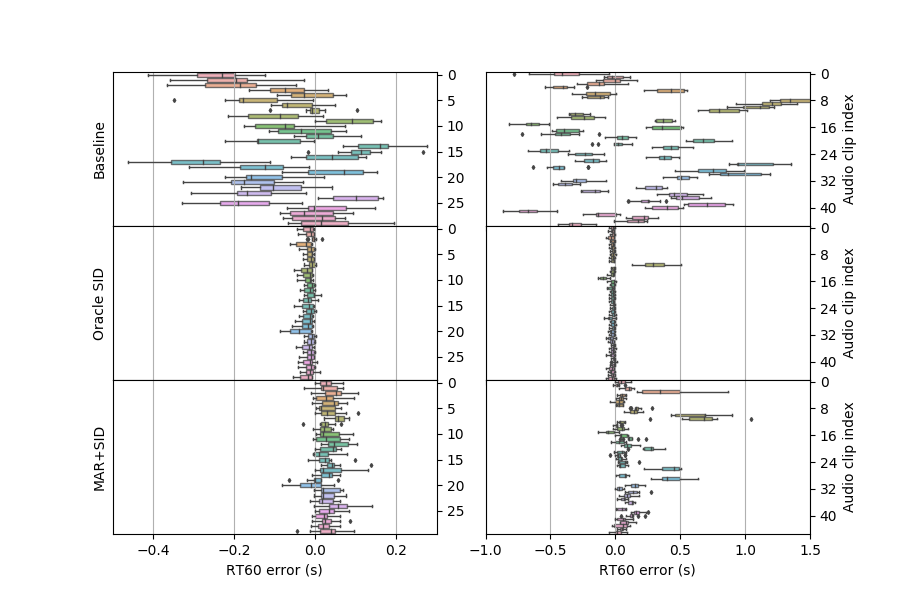
\includegraphics[width=\textwidth]{Figures/ReverberationTimeEstimation/96.png}}
%		\centerline{(a) Estimation error computed for each audio clip.}\medskip
%	\end{minipage}
%	\begin{minipage}[b]{1.0\linewidth}
%		\centerline{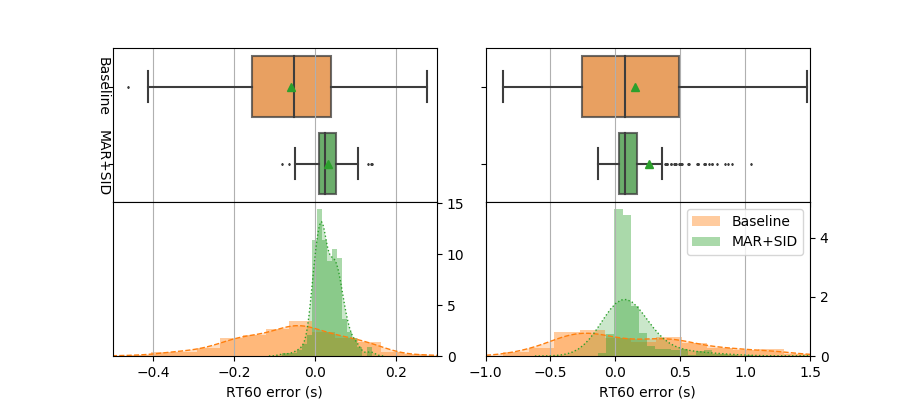
\includegraphics[width=\textwidth]{Figures/ReverberationTimeEstimation/94.png}}
%		\centerline{(b) Total estimation error across audio clips and acoustic conditions. Top: boxplot. Bottom: histogram and density plot.}\medskip
%	\end{minipage}
%	\caption{Experiment results for \textit{speech} (left column) and \textit{drums} (right column) datasets.}
%	\label{fig:results}
%\end{figure*}

\begin{figure*}[htbp]
	\centerline{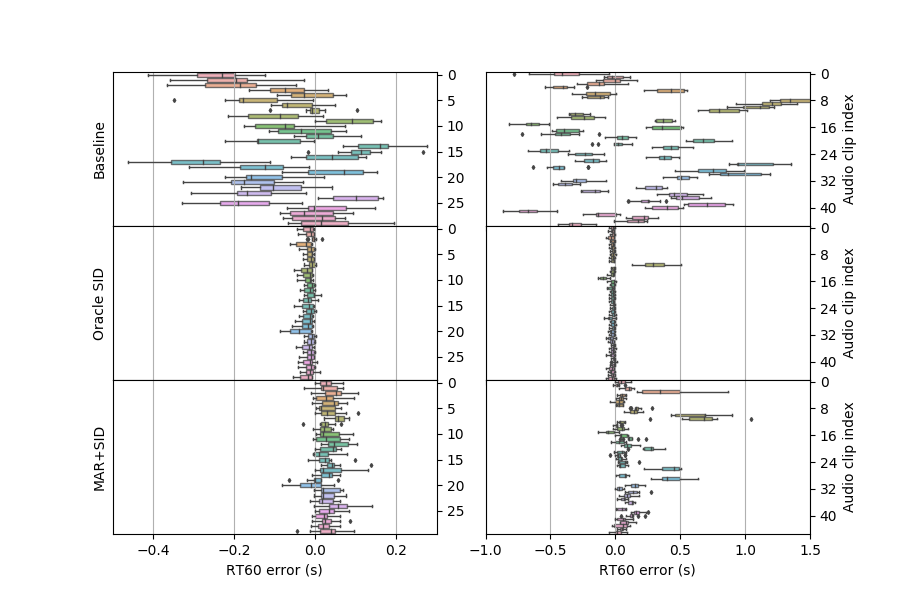
\includegraphics[width=1.1\textwidth]{Figures/ReverberationTimeEstimation/96.png}}
	\caption{Experiment results for \textit{speech} (left column) and \textit{drums} (right column) datasets. Estimation error computed for each audio clip.}
	\label{fig:results1}
\end{figure*}
\begin{figure*}[htbp]
	\centerline{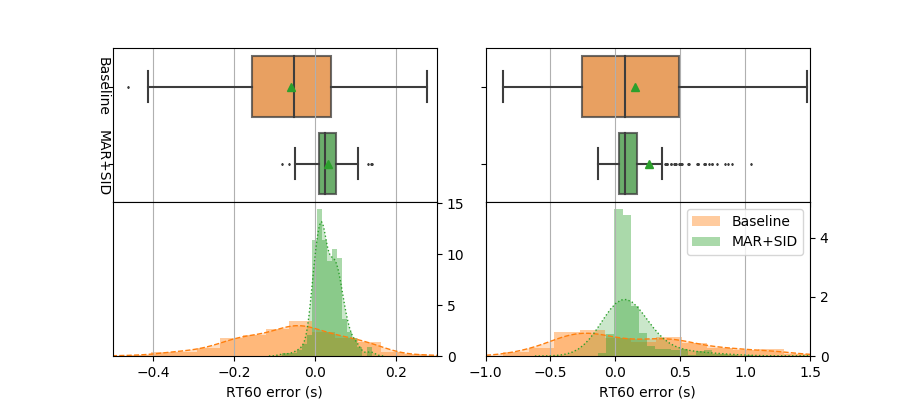
\includegraphics[width=1.2\textwidth]{Figures/ReverberationTimeEstimation/94.png}}
	\caption{Experiment results for \textit{speech} (left column) and \textit{drums} (right column) datasets. Total estimation error across audio clips and acoustic conditions. Top: boxplot. Bottom: histogram and density plot}
	\label{fig:results2}
\end{figure*}




%%%%%%%%%%%%%%%%%%%%%%%%%%%%%%%%%%%%%%%%%%%%%%%%%%%%%%%%%%%%
%%%%%%%%%%%%%%%%%%%%%%%%%%%%%%%%%%%%%%%%%%%%%%%%%%%%%%%%%%%%
\section{Conclusion}
\label{sec:conclusion}

In this Chapter, we have presented  a novel method for blind reverberation time estimation for multichannel audio, with the aim of applying it to the context of ambisonic recordings. Our method is based on a first dereverberation step,  performed by a multichannel autoregressive model of the late reverberation. The resulting dry signal is then used to estimate the impulse response decay by means of system identification. 
The performance of the method is evaluated in a simulated experimental environment with two different reverberant datasets, and compared against a state-of-the-art method. 
Results show that our method outperforms the baseline method in a majority of evaluation metrics and conditions, and consistently provides results with less variability than the baseline method. 
%In future work, we plan to extend the experimental setup by using recorded IRs. Furthermore, the proposed method could be extended to the case of moving sources by using an \textit{online} autoregressive model. 
%%Finally, an evaluation of the method in terms of the number of channels or the ambisonic order remains to be done.
%Finally, an extension of the method for higher ambisonic orders remains to be done.
